\documentclass[12pt,t]{beamer}
\usepackage{graphicx}
\setbeameroption{hide notes}
\setbeamertemplate{note page}[plain]
\usepackage{listings}
\usepackage{animate}
\usepackage{xmpmulti}
\date{} 

% header.tex: boring LaTeX/Beamer details + macros

% get rid of junk
\usetheme{default}
\beamertemplatenavigationsymbolsempty
\hypersetup{pdfpagemode=UseNone} % don't show bookmarks on initial view


% font
\usepackage{fontspec}
\setsansfont
  [ ExternalLocation = fonts/ ,
    UprightFont = *-regular ,
    BoldFont = *-bold ,
    ItalicFont = *-italic ,
    BoldItalicFont = *-bolditalic ]{texgyreheros}
\setbeamerfont{note page}{family*=pplx,size=\footnotesize} % Palatino for notes
% "TeX Gyre Heros can be used as a replacement for Helvetica"
% I've placed them in fonts/; alternatively you can install them
% permanently on your system as follows:
%     Download http://www.gust.org.pl/projects/e-foundry/tex-gyre/heros/qhv2.004otf.zip
%     In Unix, unzip it into ~/.fonts
%     In Mac, unzip it, double-click the .otf files, and install using "FontBook"

% named colors
\definecolor{offwhite}{RGB}{255,250,240}
\definecolor{gray}{RGB}{155,155,155}

\ifx\notescolors\undefined % slides
  \definecolor{foreground}{RGB}{255,255,255}
  \definecolor{background}{RGB}{24,24,24}
  \definecolor{title}{RGB}{107,174,214}
  \definecolor{subtitle}{RGB}{102,255,204}
  \definecolor{hilit}{RGB}{102,255,204}
  \definecolor{vhilit}{RGB}{255,111,207}
  \definecolor{codehilit}{RGB}{255,111,207}
  \definecolor{lolit}{RGB}{155,155,155}
\else % notes
  \definecolor{background}{RGB}{255,255,255}
  \definecolor{foreground}{RGB}{24,24,24}
  \definecolor{title}{RGB}{27,94,134}
  \definecolor{subtitle}{RGB}{22,175,124}
  \definecolor{hilit}{RGB}{122,0,128}
  \definecolor{vhilit}{RGB}{255,0,128}
  \definecolor{codehilit}{RGB}{24,24,24}
  \definecolor{lolit}{RGB}{95,95,95}
\fi
\definecolor{nhilit}{RGB}{128,0,128}  % hilit color in notes
\definecolor{nvhilit}{RGB}{255,0,128} % vhilit for notes

\newcommand{\hilit}{\color{hilit}}
\newcommand{\vhilit}{\color{vhilit}}
\newcommand{\nhilit}{\color{nhilit}}
\newcommand{\nvhilit}{\color{nvhilit}}
\newcommand{\lolit}{\color{lolit}}

% use those colors
\setbeamercolor{titlelike}{fg=title}
\setbeamercolor{subtitle}{fg=subtitle}
\setbeamercolor{institute}{fg=lolit}
\setbeamercolor{normal text}{fg=foreground,bg=background}
\setbeamercolor{item}{fg=foreground} % color of bullets
\setbeamercolor{subitem}{fg=lolit}
\setbeamercolor{itemize/enumerate subbody}{fg=lolit}
\setbeamertemplate{itemize subitem}{{\textendash}}
\setbeamerfont{itemize/enumerate subbody}{size=\footnotesize}
\setbeamerfont{itemize/enumerate subitem}{size=\footnotesize}

% page number
\setbeamertemplate{footline}{%
    \raisebox{5pt}{\makebox[\paperwidth]{\hfill\makebox[20pt]{\lolit
          \scriptsize\insertframenumber}}}\hspace*{5pt}}

% add a bit of space at the top of the notes page
\addtobeamertemplate{note page}{\setlength{\parskip}{12pt}}

% default link color
\hypersetup{colorlinks, urlcolor={hilit}}

\ifx\notescolors\undefined % slides
  % set up listing environment
  \lstset{language=bash,
          basicstyle=\ttfamily\scriptsize,
          frame=single,
          commentstyle=,
          backgroundcolor=\color{darkgray},
          showspaces=false,
          showstringspaces=false
          }
\else % notes
  \lstset{language=bash,
          basicstyle=\ttfamily\scriptsize,
          frame=single,
          commentstyle=,
          backgroundcolor=\color{offwhite},
          showspaces=false,
          showstringspaces=false
          }
\fi

% a few macros
\newcommand{\bi}{\begin{itemize}}
\newcommand{\bbi}{\vspace{24pt} \begin{itemize} \itemsep8pt}
\newcommand{\ei}{\end{itemize}}
\newcommand{\ig}{\includegraphics}
\newcommand{\subt}[1]{{\footnotesize \color{subtitle} {#1}}}
\newcommand{\ttsm}{\tt \small}
\newcommand{\ttfn}{\tt \footnotesize}
\newcommand{\figh}[2]{\centerline{\includegraphics[height=#2\textheight]{#1}}}
\newcommand{\figw}[2]{\centerline{\includegraphics[width=#2\textwidth]{#1}}}


\newcommand{\addstretch}[1]{\addtolength{#1}{\fill}}
%\newcommand\stretchy{\only<2>{%
%  \addstretch{\baselineskip}% Doesn't look very nice
  \addstretch{\abovedisplayskip}%
  \addstretch{\abovedisplayshortskip}%
  \addstretch{\belowdisplayskip}%
  \addstretch{\belowdisplayshortskip}%
  \addstretch{\parskip}%
%}}

% title info
\title{Deep Neural Nets Brass Tacks}
\author{\href{http://xyz}{Nebojsa Bozanic}}
\date{
\scriptsize {\lolit Slides:} \href{http://bit.ly/deepNets}{\tt \scriptsize
  \color{foreground} bit.ly/deepNets}
 }
\begin{document}

% title slide
{
\setbeamertemplate{footline}{} % no page number here
\frame{
  %\date{} 
  \titlepage
  
} }

%reference everything
%6x6 rule
%1 min per slide - 55
%2 tryouts
%just enough of pics/vids/links

% Abstract

%Deep Neural Networks are experiencing immense recent research resurgence, delivering
%superhuman accuracy in numerous applications. While we are witnessing its success, we fail to
%fully understand the mathematics behind deep networks. Here we'll first look at the biological and
%technological processing networks (i.e. biological inspiration for neural networks). Then, we'll take
%an overview of some state-of-the-art networks in computer vision. And at the end we will cover a
%task-tailored practical end-to-end setup of a neural network

\begin{frame}[c]{Hey}

Kindly introduce yourself

\end{frame}

\begin{frame}[c]{Brass Tacks}
%\stretchy

Brass\pause - an alloy of copper and zinc
\pause

A tack\pause - a small wide-head nail 
\pause

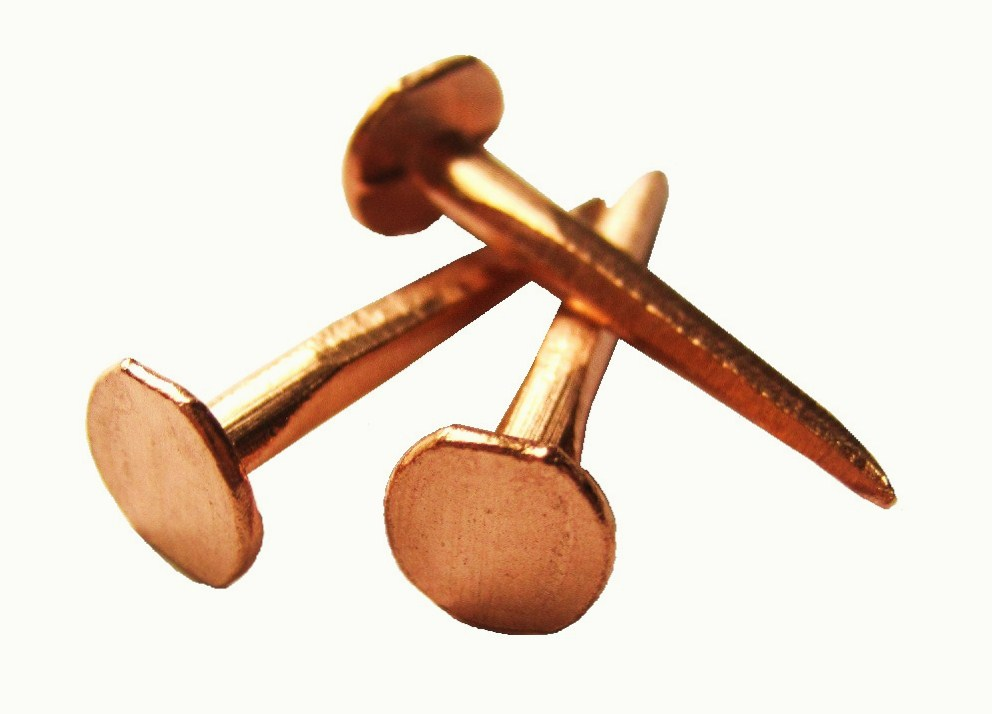
\includegraphics[height=25mm]{Figs/tacks.jpg}
\pause

Brass tacks has a meaning 
\pause
\begin{itemize}
\item Roll up one's sleeves
\pause
\item Get down to business 
\pause
\item \textbf{Deal with the important details}
\end{itemize}

\end{frame}

\begin{frame}[c]{An ambitious goal}

%The purpose is not to be yet another theoretical talk

\pause
Everyone that knows nothing or have a partial knowledge about Deep Learning should be able to use state-of-the-art DNN models

\end{frame}

\begin{frame}[c]{Today's to do list}

\pause
1. What are Deep Neural Networks?
\pause

2. Their Performance?
\pause

3. How to use them in my research/production?


\end{frame}

\begin{frame}[c]{Deep Neural Networks}

What is a 'Neural Network' in Deep Neural Networks?

%biological processing network to technological one
%The mathematics behind deep networks?
\end{frame}

\begin{frame}[c]{Neural Networks}

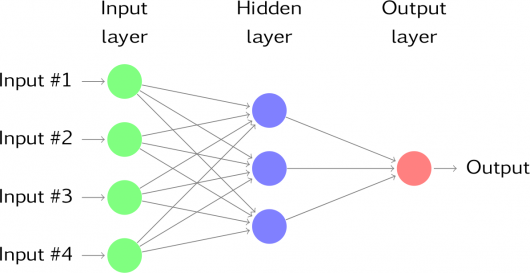
\includegraphics[height=45mm]{Figs/neuralnet.png}

"A Neural Network is inspired by our knowledge the inner-workings of the human brain."

%\note{"A NN is a very loose model of the human brain that we can program in the computer. Or it's perhaps more appropriate to say that it is inspired by our knowledge the inner-workings of the human brain."}

\hfill
{\footnotesize \lolit
\href{https://www.youtube.com/watch?v=He4t7Zekob0}{\tt How Does Deep Learning Work? Two Minute Papers \# 24 by Karoly Zsolnai Feher}
}

\end{frame}

\begin{frame}[c]{Neural Networks}
\animategraphics[loop,controls,width=\linewidth]{12}{Figs/gif/frame_}{0}{210}

\end{frame}

\begin{frame}[c]{Neural Networks}
\animategraphics[loop,controls,width=\linewidth]{12}{Figs/gif/frame_}{0}{1}

{\footnotesize \lolit
\href{https://www.youtube.com/watch?v=QSaZGT4-6EY}{\tt  Deep Learning for Intelligent Computer Systems by Jeff Dean}
}

\end{frame}

\begin{frame}{Neural Nets}

Let's take a look first at two examples of sensory processing networks; \pause

One is technological, the other is biological; \pause

Both handle visual information. \pause

\end{frame}

\begin{frame}{Biological Inspiration}
Ramón y Cajal’s Retina

  
Mammalian retinal structure –  note the apparent layers that are very clearly depicted.  Different anatomical Layers are associated with different functional properties of cells.  

The \textit{layered} structure is typical of neural circuitry involved in sensory perception.  


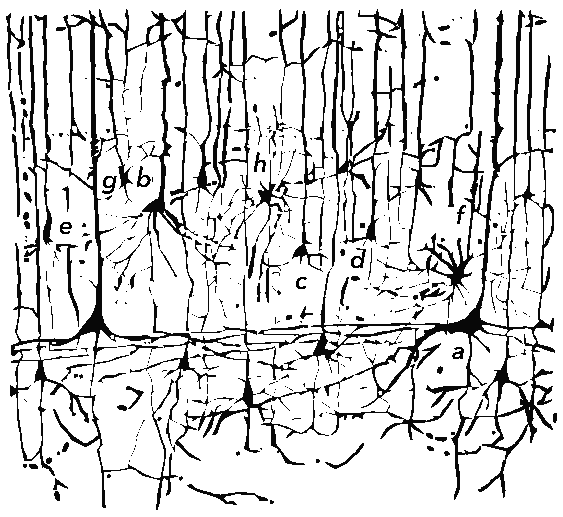
\includegraphics[height=30mm]{Figs/ramonycajal.pdf}
c.1900 By Santiago Ramón y Cajal.  
 
\end{frame}

\begin{frame}[c]{Biological Inspiration}

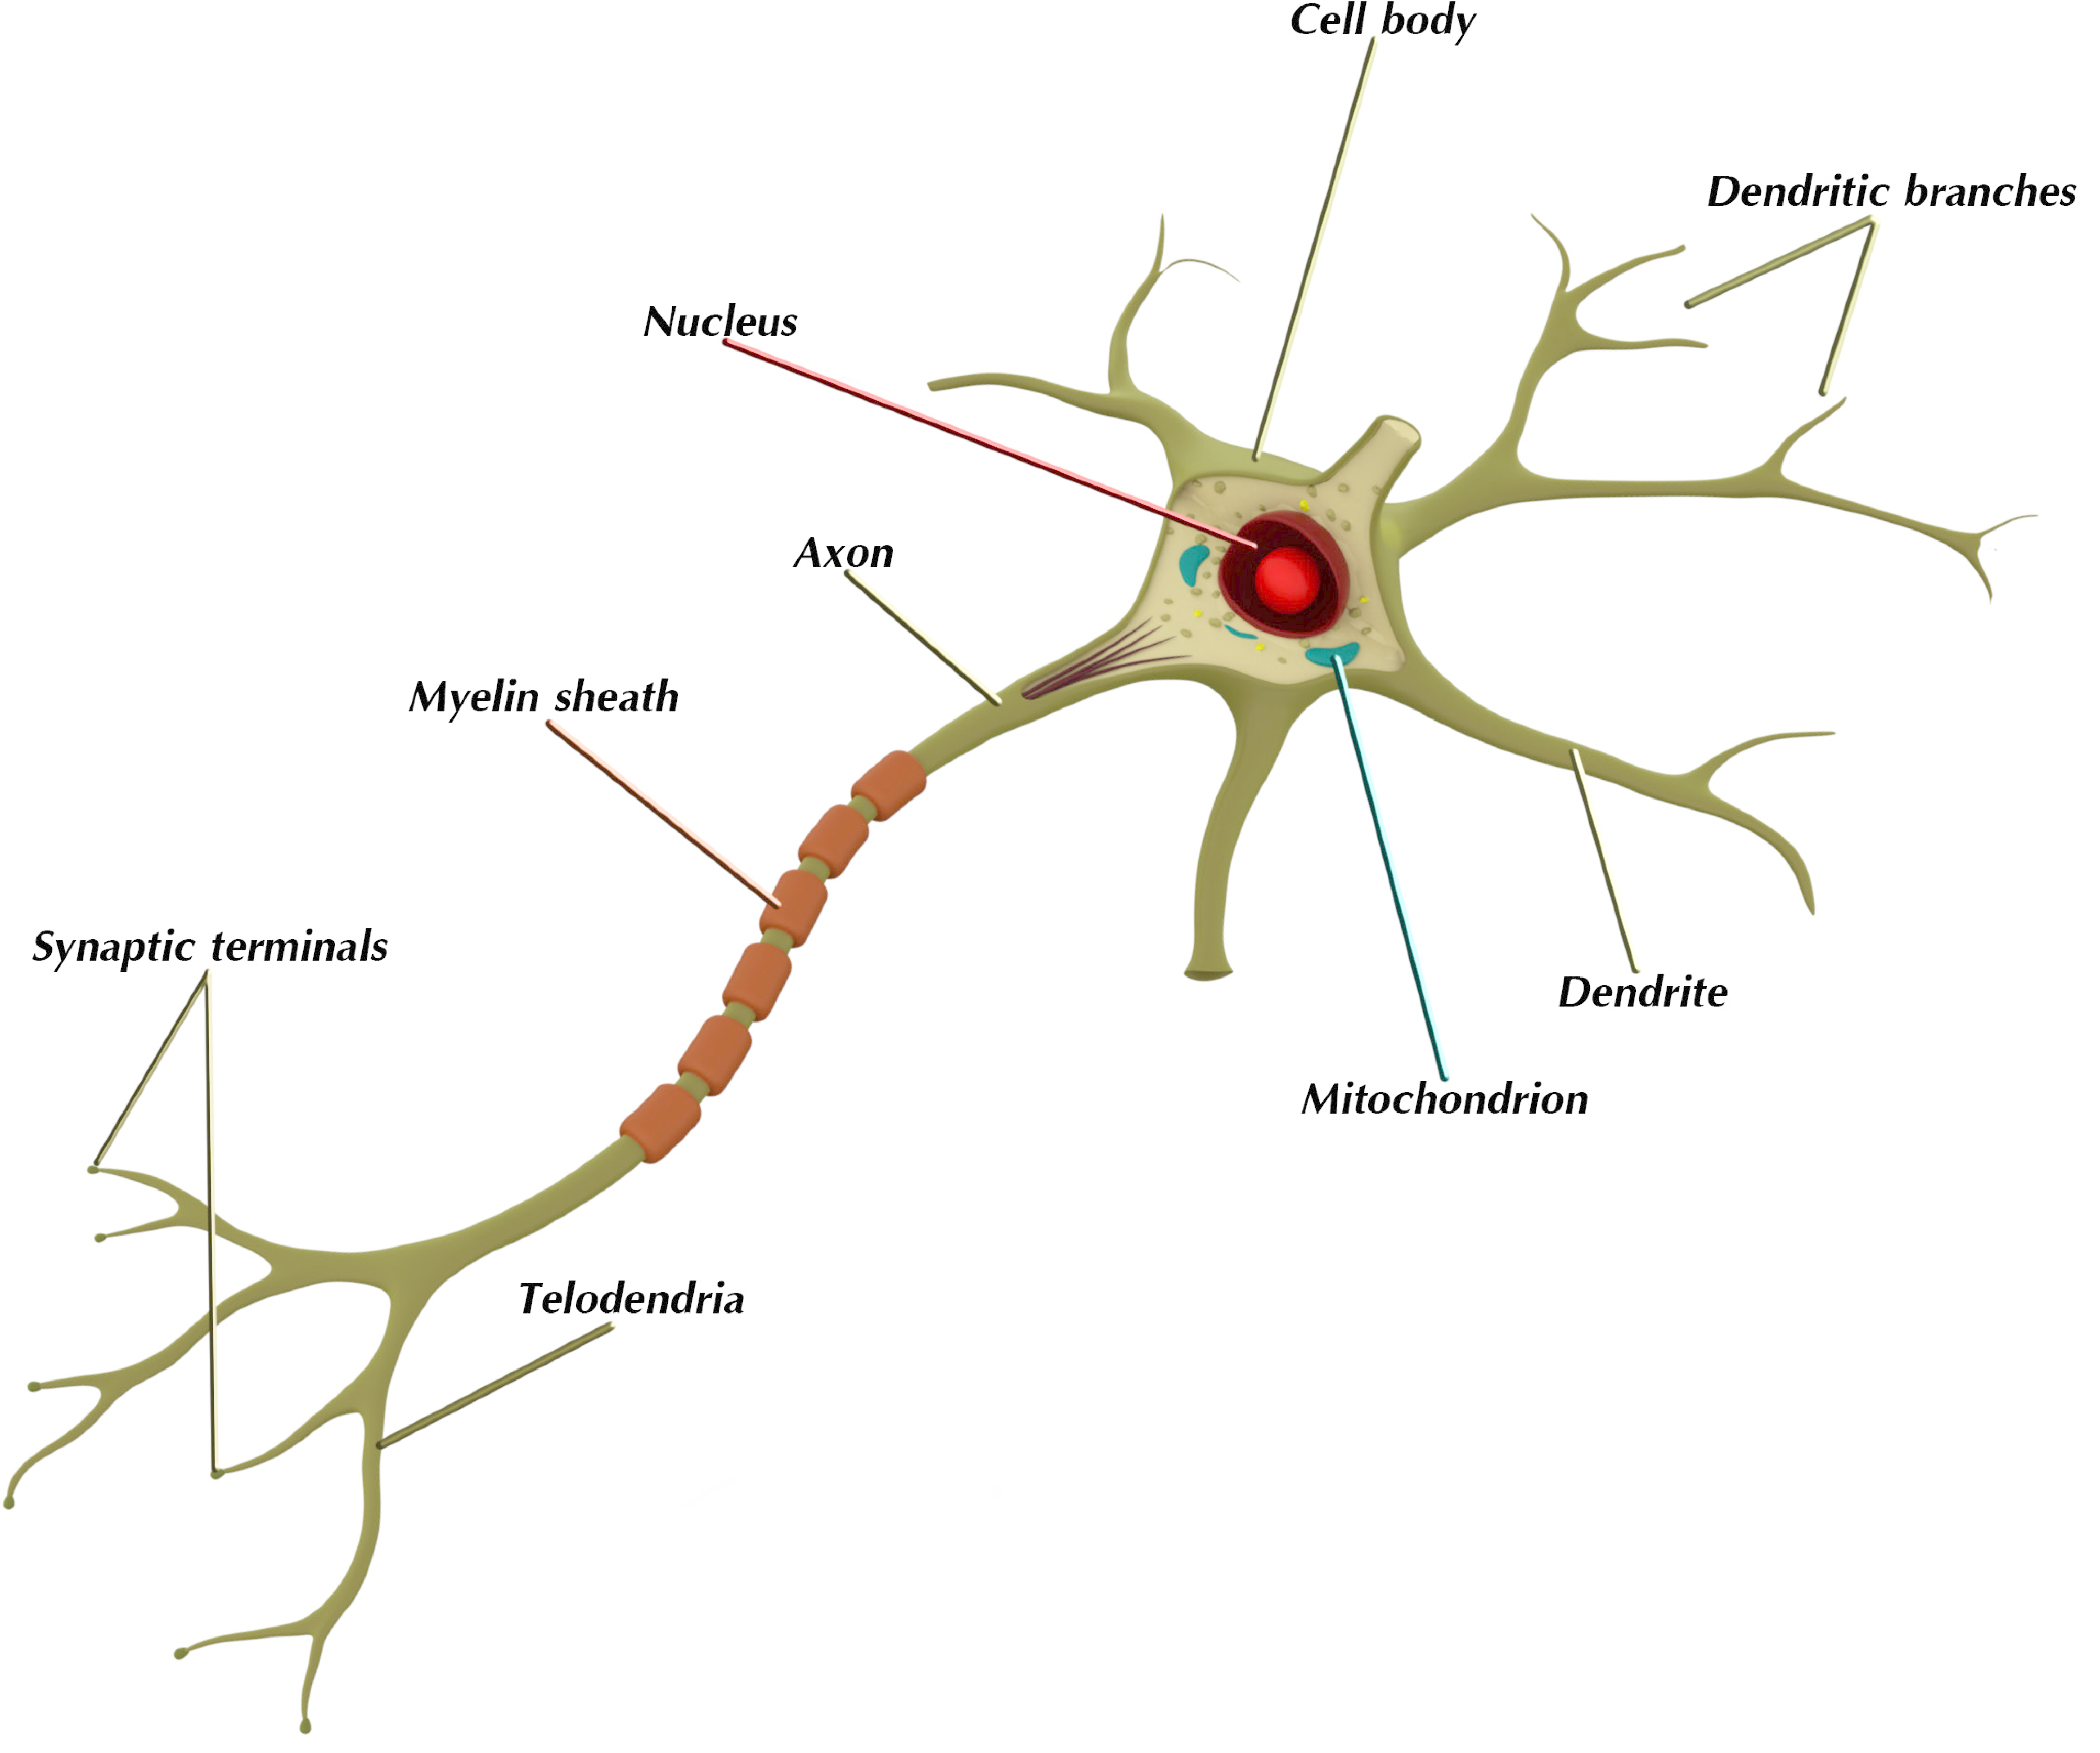
\includegraphics[height=60mm]{Figs/complete_neuron.pdf}

\hfill
{\footnotesize \lolit
{\tt A Neuron}
}

\end{frame}

\begin{frame}{The Complexity of Vision}

Some 'statistics' on the human retina: 

\begin{itemize}
\item 120 million photoreceptors in each human retina.

\item Approximately 5 distinct layers of cells.

\item Various areas of the retina: 

	\begin{itemize}
	\item Central Fovea
	
	\item Fovea

	\item Periphery 
 
	\end{itemize} 

\item Variation of properties/ratios of photoreceptors/ganglion cells across the retina. 

\end{itemize} 
 
\end{frame}

\begin{frame}[c]{Receptive fields}

Spike-triggered averaging (STA) – also known as reverse 'correlation': a probabilistic characterisation of receptive fields.

 Run through a random series of spatial patterns, and empirically estimate:
	\begin{itemize}
	\item – P(spike|spatial pattern stimulus; t)
	\end{itemize}

Provides a systematic way of capturing response characteristics of cells.

\end{frame}

\begin{frame}[c]{The 'Optimal' Stimulus}

\begin{itemize}

\item A visual Interpretation of a retinal receptive Field

	\begin{itemize}

	\item The 'optimal visual stimuli': probability of firing of two classes of retinal ganglion cells might be highest for these stimuli*.
	\item Examples:
	
OFF Centre
ON Centre

*This is a simplified, but 'on average' response.

	\end{itemize}
\end{itemize}

\end{frame}

\begin{frame}[c]{Visual Information: The Path}

Retina -> LGN -> V1 -> Projections to other brain areas;

Anatomically distinct brain regions that can be captured by painstaking histopathology (for example, see Van Essen’s work);

\hfill
{\footnotesize \lolit
\href{http://bicv.org/downloads/Shallow_Introduction_to_Deep_Learning-Jan_30_2014.pdf}{\tt Shallow Introduction to Deep Learning. Anil Bharath}
}

\end{frame}

\begin{frame}[c]{Visual Information: The Path}

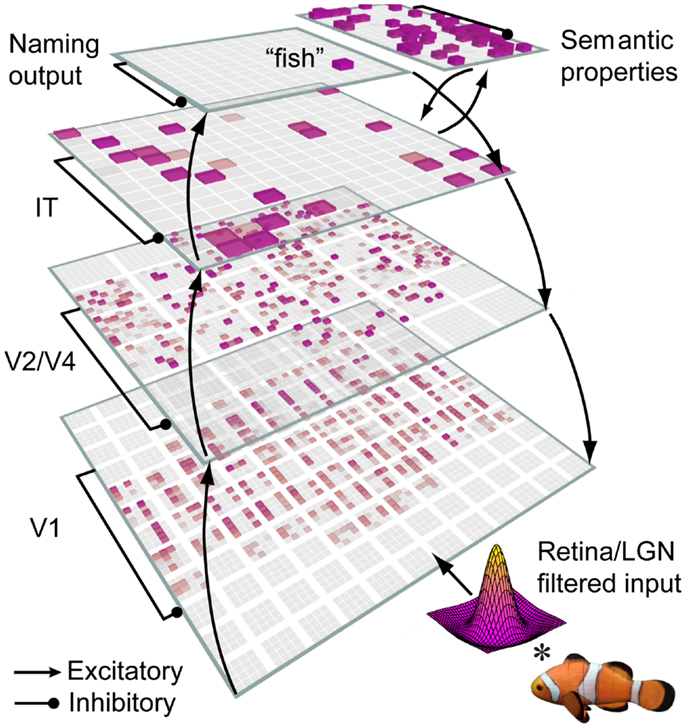
\includegraphics[height=70mm]{Figs/biological_visual_pathway.jpg}

\hfill
{\footnotesize \lolit
\href{http://journal.frontiersin.org/article/10.3389/fpsyg.2013.00124/full}{\tt Biological architecture of a visual pathway}
}

\end{frame}

\begin{frame}[c]{Visual Information: The Path}

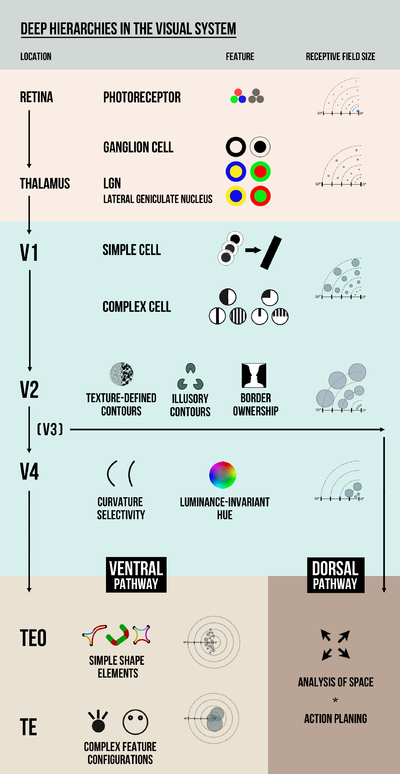
\includegraphics[height=80mm]{Figs/visual_system_hierarchies.png}

\hfill
{\footnotesize \lolit
\href{https://en.wikibooks.org/wiki/Sensory_Systems/Visual_System}{\tt Wiki Books - Visual System}
}

\end{frame}

\begin{frame}[c]{Cortical Layers}


Cortex uses layered architecture for different types of function.

For vision, we know that we can associate different visual receptive field properties with different layers;

Staining for cell bodies in (left) visual cortex and (right) motor cortex of human adult. From Santiago Ramón y Cajal 'Comparative study of the sensory areas of the human cortex', 1899. Reprinted by Nabu Press, 2010.

\end{frame}

\begin{frame}

Possible, though not easy to experimentally find receptive fields for higher visual areas.

However, we do not suggest a grandmother cell so much as a joint encoding of visual structure by many cells.

Rough idea of selectivity to properties; however, selectivity is usually 'soft' and not 'hard':
e.g. orientation tuning curves.

\end{frame}

\begin{frame}

And now, the machines…

\end{frame}

\begin{frame}[c]{A Neuron Model}

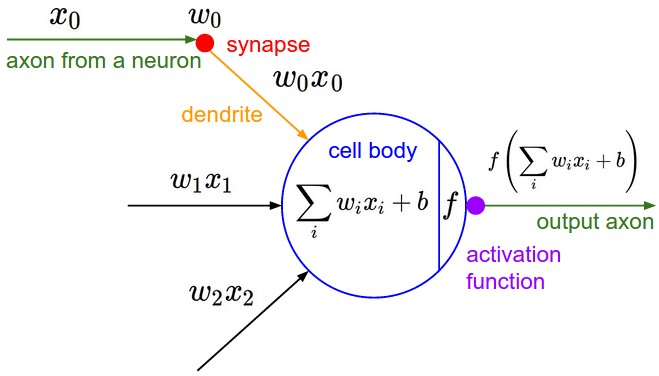
\includegraphics[height=40mm]{Figs/neuron_model.jpeg}

\hfill
{\footnotesize \lolit
\href{http://cs231n.github.io}{\tt Stanford CS class by Andrej Karpathy}
}

\end{frame}

\begin{frame}[c]{Activation Function}

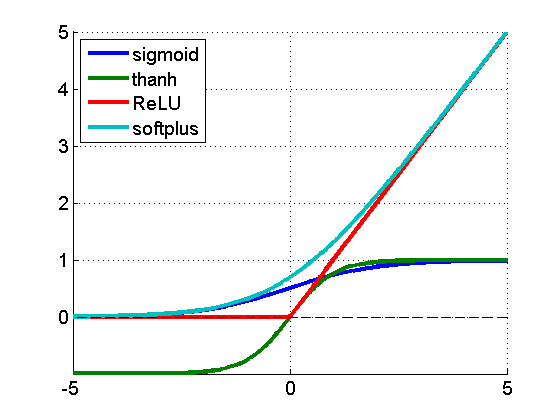
\includegraphics[height=45mm]{Figs/activations.png}

\hfill
{\footnotesize \lolit
\href{http://cs231n.github.io/convolutional-networks/}{\tt Stanford CS class by Andrej Karpathy}
}

\end{frame}


\begin{frame}[c]{1D Convolutional Network}

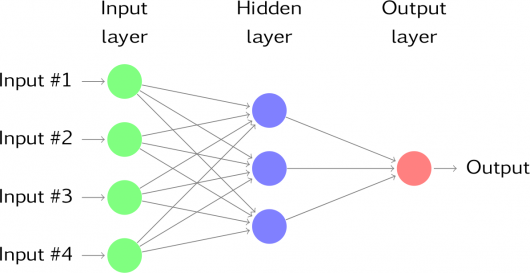
\includegraphics[height=45mm]{Figs/neuralnet.png}

\hfill
{\footnotesize \lolit
{\tt 1D Network}
}

\end{frame}

\begin{frame}[c]{2D Convolutional Network}

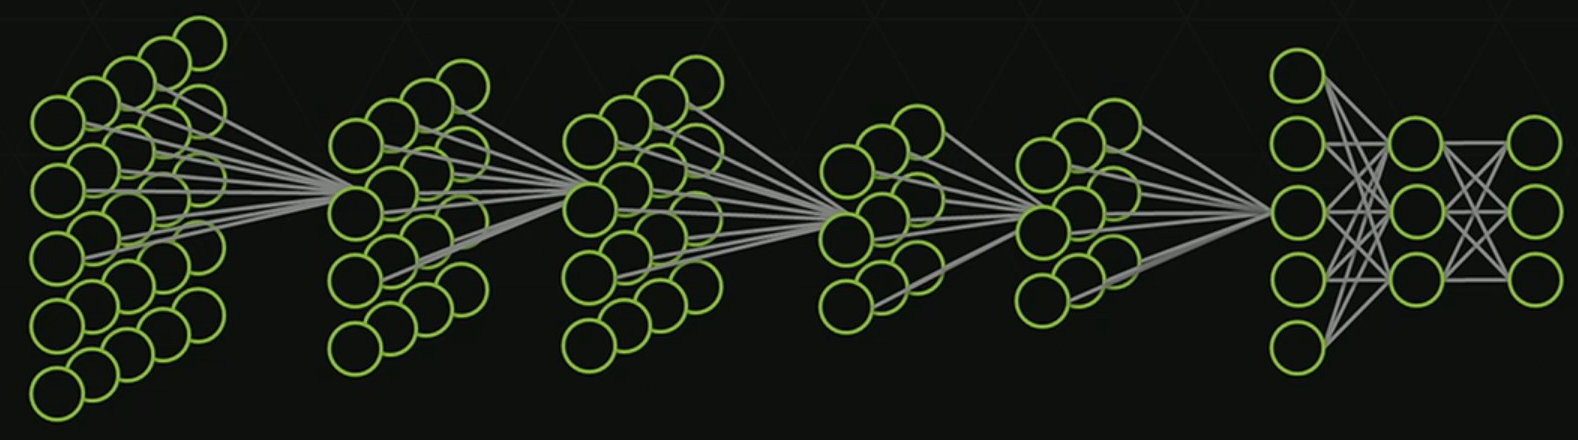
\includegraphics[height=25mm]{Figs/nvidia.jpg}

\hfill
{\footnotesize \lolit
{\tt 2D Network}
}

\end{frame}

\begin{frame}[c]{Analyzing results}

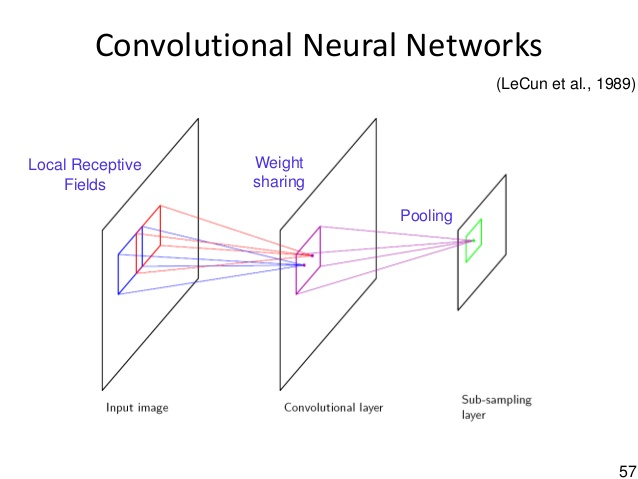
\includegraphics[height=60mm]{Figs/LeCun1989.jpg}

\hfill
{\footnotesize \lolit
\href{http://yann.lecun.com/exdb/publis/pdf/lecun-89e.pdf}{\tt LeCun ConvNets, ICML 1989}
}

\end{frame}

\begin{frame}[c]{Convolutional Multilayer Network}

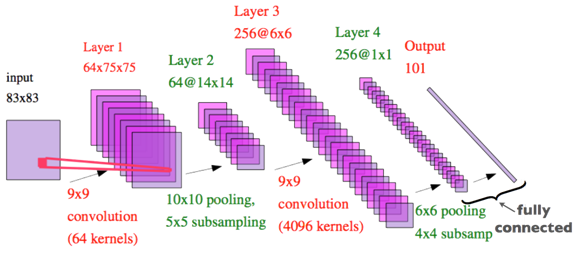
\includegraphics[height=45mm]{Figs/multilayer.png}

\hfill
{\footnotesize \lolit
{\tt LeCun ConvNets, ICML 2012 }
}

\end{frame}

\begin{frame}[c]{(Matrix) Convolution}

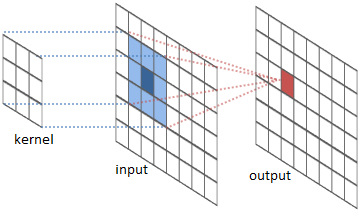
\includegraphics[height=35mm]{Figs/convolution.png}

\hfill
{\footnotesize \lolit
\href{http://cs231n.github.io/convolutional-networks/}{\tt Stanford CS class by Andrej Karpathy}
}

\end{frame}

\begin{frame}[c]{Max Pooling}

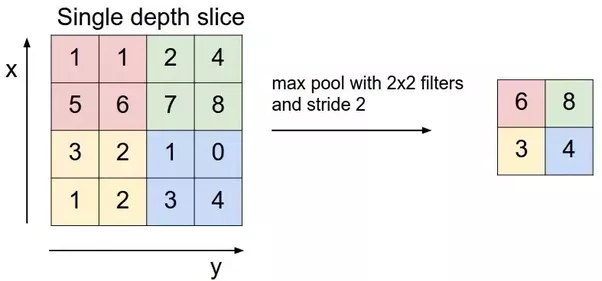
\includegraphics[height=40mm]{Figs/maxpool.png}

\hfill
{\footnotesize \lolit
\href{http://cs231n.github.io/convolutional-networks/}{\tt Stanford CS class by Andrej Karpathy}
}

\end{frame}

\begin{frame}

Let's try again...

Deep Learning systems

Multi-layered networks of units, that are based on simple artificial neurons, which encode and classify sensory data.

Start with the single artificial neuron to revise some terminology and concepts;
\end{frame}


\begin{frame}

Objectives in training a DNN

\begin{itemize}

\item Accurately encoding 'stimuli'

	\begin{itemize}

	\item generally, at the lower levels of the network
	\item classifying accurately at the top level
	
	\end{itemize}

\item Sparsity: all levels – not all units are ac0ve in response to stimuli from the layer below;
\item Robustness to noise (e.g. denoising autoencoder), usually at the lower level(s), but see MacKay for a more general view of neuronal capacity in the noisy channel-coding sense.

\end{itemize}

\end{frame}

\begin{frame}

Convolutional Deep Learning Systems

\begin{itemize}

\item Training on small patches (non-convolutional) leads to good performance, particularly if:
	
	\begin{itemize}
	\item There is no clutter in the images;
	\item The objects are centered in the field of view; 
	\item The field of view is small;
	\end{itemize}
	
\item Recently, convolutional deep learning systems have been used by the DL community very successfully.
\item Some debate about benefits of convolutional networks vs non-convolutional; experimental results are pretty convincing, though.

\end{itemize}
\end{frame}

\begin{frame}[c]{Capacity}

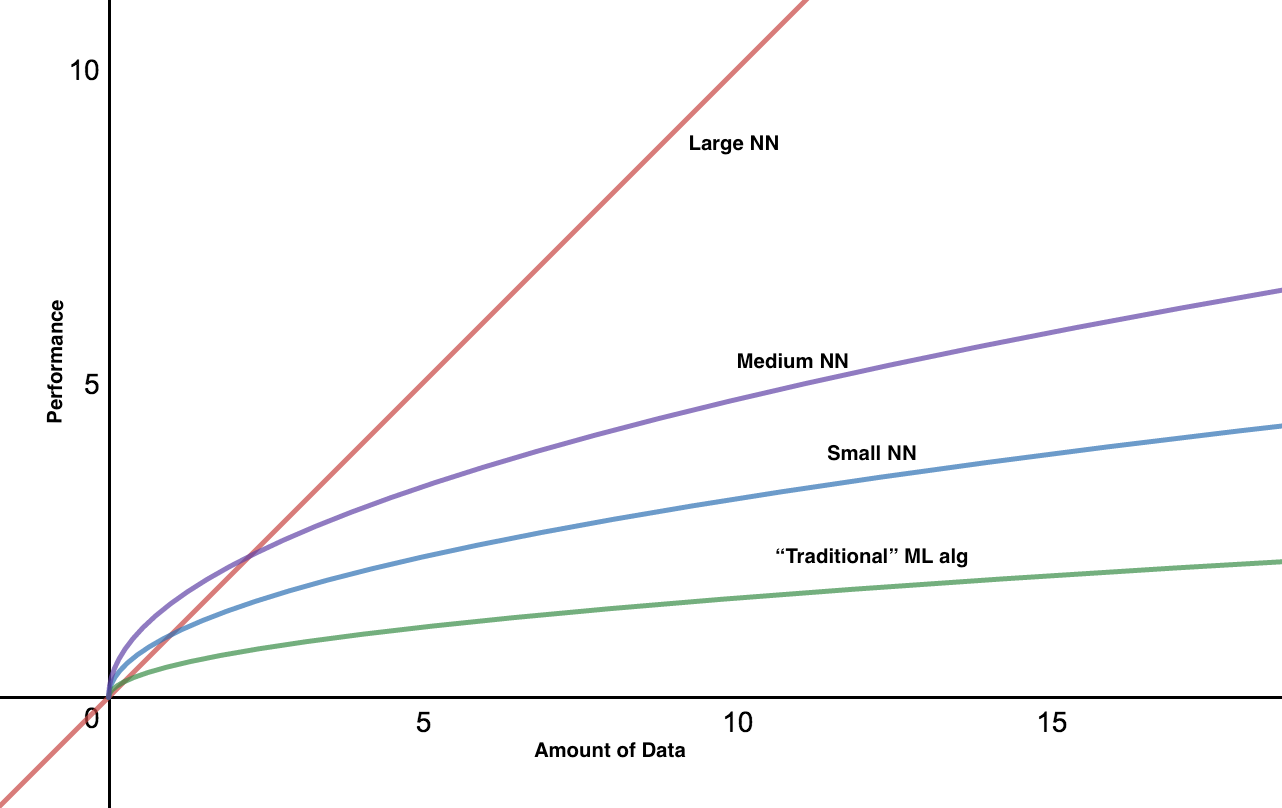
\includegraphics[height=60mm]{Figs/performance.png}

\hfill
{\footnotesize \lolit
\href{https://www.youtube.com/watch?v=F1ka6a13S9I}{\tt Nuts and Bolts of Applying Deep Learning Andrew Ng at Deep Learning School }
}

\end{frame}


\begin{frame}[c]{Deep Neural Networks}

\pause

Why 'deep' in Deep Neural Networks?

\end{frame}

\begin{frame}[c]{Deep Neural Networks}

	\begin{itemize}
	\item A Deep Neural Networks (DNN) system contains multiple hidden layers of network between input and output layers;

	\item DNN systems are reminiscent of multi-layer perceptrons, BUT:

		\begin{itemize}
		\item DNN systems are often trained by exploiting both  \textbf{supervised} and  \textbf{unsupervised} training in the same network;

		\item DNN systems may mixed architectures from layer to layer, that often conform to hybrid probabilistic models;

		\item Training regimes may differ depending on layer, reflecting a balance between the need to represent and to classify data

		\end{itemize}
	\end{itemize}
	
\end{frame}

\begin{frame}[c]{Architecture: Inception}

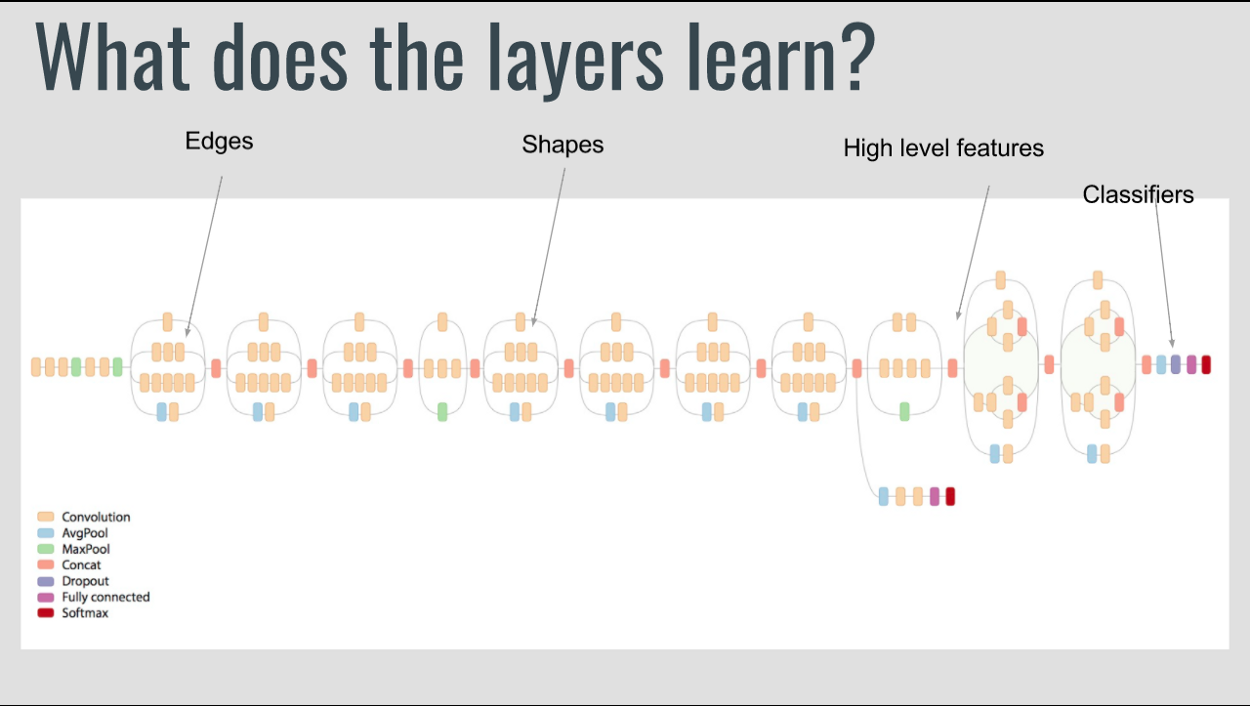
\includegraphics[height=60mm]{Figs/inception_v3_visual_representation.png}

Google Inception V3 model

\hfill
{\footnotesize \lolit
\href{https://research.googleblog.com/2016/03/train-your-own-image-classifier-with.html}{\tt Inception V3}
}

\end{frame}

\begin{frame}[c]{Architectures / Models}

\pause

what is a Neural Model?
\pause

\end{frame}

\begin{frame}{Acronyms}

Deep Neural Networks \pause

\begin{itemize}

\item DLN: Deep Learning Network \pause
\item DL: Deep Learning (refers to the field of study) \pause
\item DBN: Deep Belief Network \pause
\item DBM: Deep Boltzmann Machine \pause
\item RBM: Restricted Boltzmann Machine \pause
\item CNN: Convolutional Neural Network \pause
\item HTM: Hierarchical Temporal Memory \pause
\item MSC: Map Seeking Circuit \pause

\end{itemize}

\end{frame}

\begin{frame}[c]{Performance}

\pause

Deep Neural Networks are experiencing immense recent research resurgence
\pause

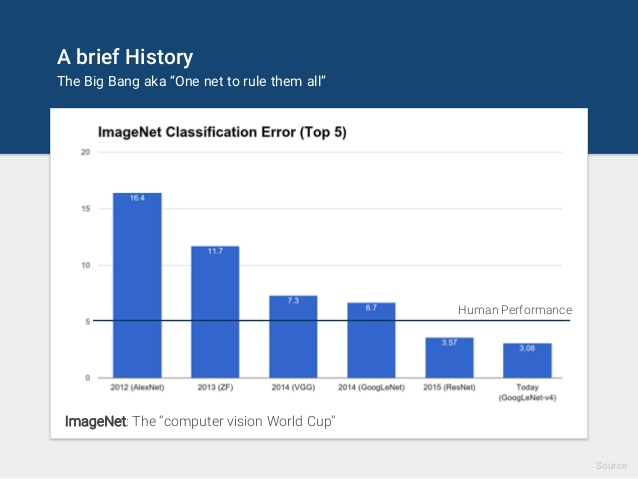
\includegraphics[height=60mm]{Figs/performance_imagenet_years.jpg}
\pause

\href{http://papers.nips.cc/paper/4824-imagenet-classification-with-deep-convolutional-neural-networks.pdf}{Krizhevsky et al. 2012: AlexNet}
\pause

\hfill
{\footnotesize \lolit
\href{http://www.image-net.org/challenges/LSVRC}{\tt ImageNet Classification Challenge}
}

\end{frame}

\begin{frame}[c]{Performance}

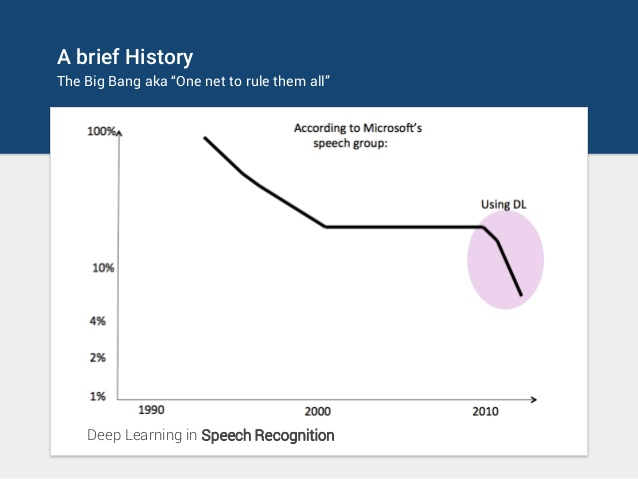
\includegraphics[height=60mm]{Figs/performance_speech_year.jpg}
\pause

Superhuman accuracy in Face Verification
\pause

facenet 99.63\% (on lfw dataset)  
\href{http://www.cv-foundation.org/openaccess/content_cvpr_2015/app/1A_089_ext.pdf}{FaceNet}
\pause
\end{frame}

\begin{frame}[c]{Setup}

%In order to use DNN one would need to consider using one of the following frameworks/IDE/...
\pause

To use a DNN
\pause

- get a framework
\pause

- (debug) IDE (integrated development environment
\pause

- (optional) GPU (NVIDIA graphic card)
\pause

- (optional) Server
 
\end{frame}

\begin{frame}[c]{ Frameworks - Part I}

%https://medium.com/@ricardo.guerrero/deep-learning-frameworks-a-review-before-finishing-2016-5b3ab4010b06
\pause

\href{https://www.tensorflow.org/}{Tensorflow}
\pause

\href{http://deeplearning.net/software/theano/}{Theano}
\pause

\href{https://keras.io/}{Keras}
\pause

\href{http://lasagne.readthedocs.io/en/latest/index.html}{Lasagne}
\pause

\href{http://caffe.berkeleyvision.org/}{Caffe}

\end{frame}

\begin{frame}[c]{Frameworks - Part II}

%https://medium.com/@ricardo.guerrero/deep-learning-frameworks-a-review-before-finishing-2016-5b3ab4010b06
\pause

\href{https://github.com/amzn/amazon-dsstne}{DSSTNE}
\pause

\href{http://torch.ch/}{Torch}
\pause

\href{https://github.com/dmlc/mxnet}{mxnet}
\pause

\href{https://deeplearning4j.org/}{DL4J}
\pause

\href{https://github.com/Microsoft/CNTK}{Cognitive Toolkit}
\pause

\hfill
{\footnotesize \lolit
\href{https://medium.com/@ricardo.guerrero/deep-learning-frameworks-a-review-before-finishing-2016-5b3ab4010b06}{\tt Deep Learning Frameworks - A Review}
}

\end{frame}


\begin{frame}[c]{Python IDEs}

\pause

\href{https://www.jetbrains.com/pycharm/}{PyCharm}
\pause

VIM
\pause

\href{http://www.pydev.org/}{Pydev}
\pause

\href{https://pythonhosted.org/spyder/}{Spyder Python}
\pause

\href{http://thonny.org/}{Thonny}  \pause , \href{https://www.activestate.com/komodo-ide}{Komodo IDE} \pause , \href{https://www.sublimetext.com/3}{Sublime Text} \pause ...

\end{frame}

\begin{frame}[c]{Task-Tailored Practical End-to-End Setup of a Neural Network}

\pause

Let's build an image classifier %in 30 lines of python that has a 99 percent of accuracy
\pause

Choose an object you want to classify
\pause

We can choose to:
\pause

\begin{itemize}
\item train a cnn ourselves
\pause

\begin{itemize}
\item computer power
\pause

\item lots of time
\pause
 
\end{itemize}
%if we want to train cnn ourselves we would need a lot of computing power and lot of time
\pause

or 
\pause

\item use a pretrained model
% that's why we wanna use a pretrained cnn model called inception. inception is trained by google on 100k images with a 1000 categories.

\end{itemize}

\end{frame}

\begin{frame}[c]{Build a Classifier}

\pause

Object: X
\pause

Pretrained model: \pause
\begin{itemize}
\item  Inception V3 \pause
	\begin{itemize}
		\item trained on 1.2m images, 1000 classes, training took 2 weeks on a google computer with 8 GPUs
	\end{itemize}
\end{itemize}
\pause

What if Inception was not trained on Object X?
\pause

\begin{itemize}

%So gonna perform a process called 
\item Transfer learning
\pause

	\begin{itemize}

	% That means 
	\item Applying learnings from a previous training session to a new training session
	\end{itemize}

\end{itemize}

\end{frame}

\begin{frame}[c]{Building a Classifier (Steps)}

\pause

\begin{itemize}

\item 1. Install Tensorflow 
\pause
\begin{itemize}

\item (if you one is a newbie in Tensorflow/Python, install it with Keras) \pause

\end{itemize}
\item 2. Download (get) Dataset
\pause	
\begin{itemize}

\item	link tf image to Dataset	\pause

\end{itemize}
%	create a folder 
%	mkdir tf_files
%	mkdir tf_files/xxx
%	cd tf_files_xxx
	
\item 3. Download Training Script
\pause
\begin{itemize}
	
\item	git pull 	\pause

\end{itemize}

\item 4. Retrain model
\pause

\item 5. Classify
\pause

\end{itemize}

\hfill
{\footnotesize \lolit
\href{https://www.youtube.com/watch?v=QfNvhPx5Px8}{\tt 1. Build a TensorFlow Image Classifier in 5 Min by Siraj Raval}
}	
	
\end{frame}
 
\begin{frame}[c]{Building a Classifier}

\pause

What if there are more objects?
\pause

Difference between objects  X and Y?
\pause

or n objects?
\pause

repeat step 2. Download (get) dataset and link it
\pause

run retrain.py
\pause

\hfill
{\footnotesize \lolit
\href{https://www.youtube.com/watch?v=cSKfRcEDGUs}{Train an Image Classifier with TensorFlow for Poets by Josh Gordon}
}	


\end{frame}

\begin{frame}[c]{Obtaining Results}

\pause

85 - 99\% accuracy
\pause

and then what?
\pause

Accuracy:
\begin{itemize}
	\item Model (Training Set) / Cross-Validation \pause
	\item Validation \pause
	\item Test \pause
		\begin{itemize}
		\item Overall accuracy (ROC, PR)
		\end{itemize}
\end{itemize} 

\end{frame}

\begin{frame}[c]{Analyzing results}

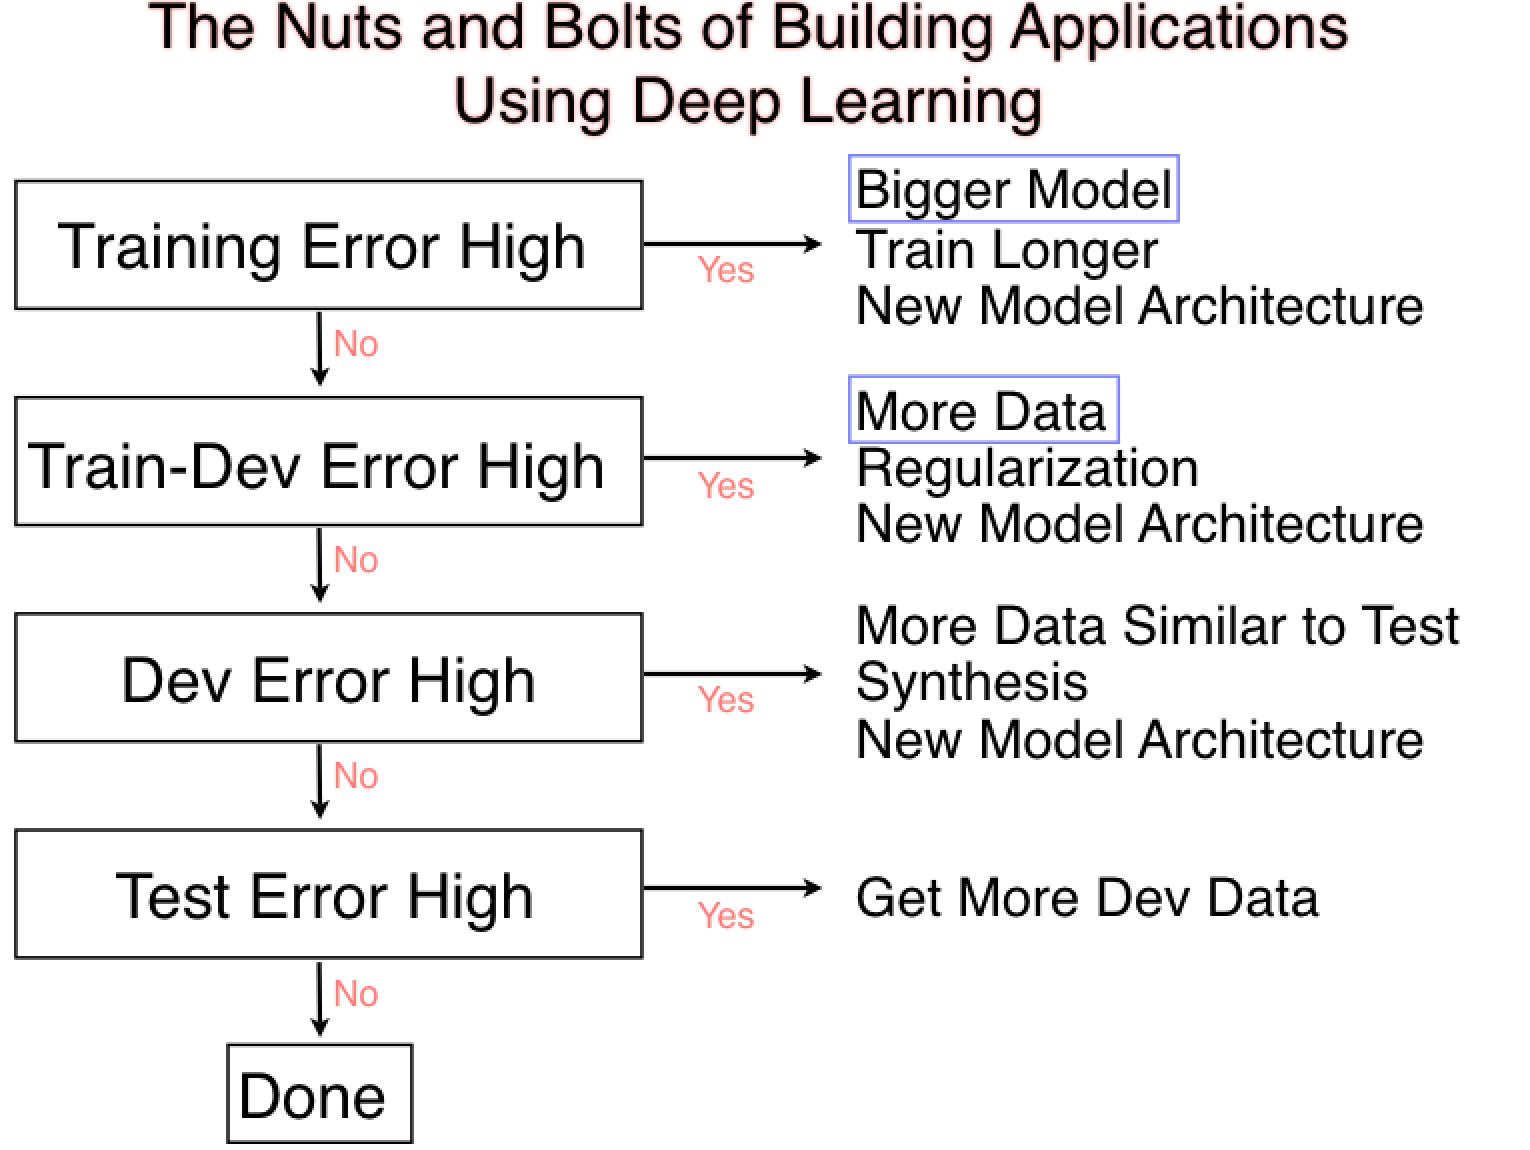
\includegraphics[height=60mm]{Figs/checklist.png}

\hfill
{\footnotesize \lolit
\href{https://www.youtube.com/watch?v=F1ka6a13S9I}{\tt Nuts and Bolts of Applying Deep Learning Andrew Ng at Deep Learning School }
}

\end{frame}

\begin{frame}[c]{A good recipe}

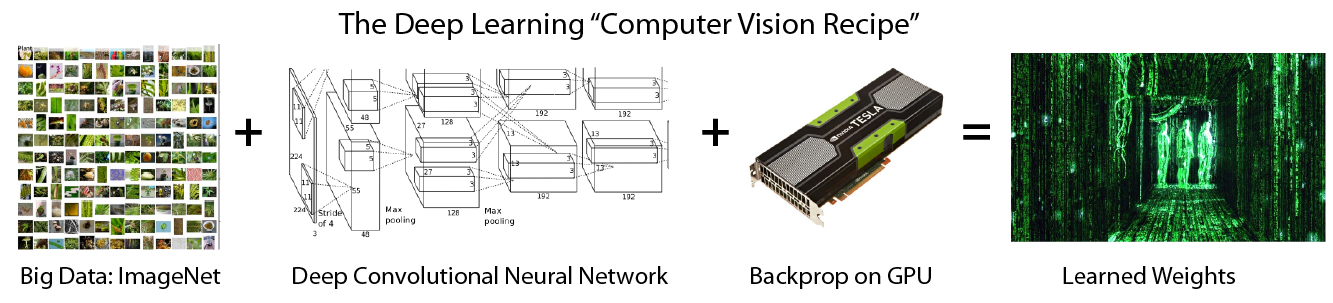
\includegraphics[height=25mm]{Figs/pipeline.png}

\hfill
{\footnotesize \lolit
\href{http://www.computervisionblog.com/2015/05/deep-learning-vs-big-data-who-owns-what.html}{\tt Pipeline }
}

\end{frame}

\begin{frame}

Bibliography \& Suggested Reading

\href{http://vision.stanford.edu/teaching/cs231n/syllabus.html}{Stanford Course: Convolutional Neural Networks for Visual Recognition}
Karpathy 

\begin{itemize}
 
\item For starters: 
 
	\begin{itemize}

	\item Bengio, Y., 'Learning Deep Architectures for AI', Foundations and Trends in Machine Learning Vol. 2, No. 1 (2009) 1–127, DOI: 10.1561/2200000006.
	\item David J.C. MacKay, 'Information Theory, Inference, and Learning Algorithms', CUP, 2006, for brushing up on single neuron models, learning rules and links between statistics and physics. 
	\item NIPS 2010 tutorial

	\end{itemize}
	
\end{itemize}

\end{frame}

\begin{frame}

Links:

\href{http://bicv.org/downloads/Shallow_Introduction_to_Deep_Learning-Jan_30_2014.pdf}{Anil Bharath: Shallow Introduction to Deep Learning} 

\href{https://media.nips.cc/Conferences/2016/Slides/6203-Slides.pdf}{Andrew Ng: Nuts and bolts of building AI applications using Deep Learning}

\href{https://kbroman.wordpress.com/2013/10/07/better-looking-latexbeamer-slides/}{kbroman Beamer Presentation Template}

\href{https://codelabs.developers.google.com/codelabs/tensorflow-for-poets}{Tensorflow For Poets}
 
\href{ https://github.com/tensorflow/models}{Tensorflow Models GitHub Repo}

\href{https://research.googleblog.com}{Google Research Blog on Tensorflow Models}
 
\end{frame}

\begin{frame}[c]{Skipped Theoretical}

Initialization

Regularization

Backpropagation

Softmax

Fully conected layers

\end{frame}

\begin{frame}[c]{Skipped Practical}

Data Augmentation

\href{https://arxiv.org/pdf/1412.1897.pdf}{DNN can be easily fooled}

\href{https://www.tensorflow.org/get_started/summaries_and_tensorboard}{Tensorboard}

\href{http://proceedings.mlr.press/v48/santoro16.pdf}{Training with less data }
\begin{itemize}
\item Meta Learning
	\begin{itemize} 
	\item One Shot Learning
	\end{itemize}
\end{itemize}

\end{frame}

\end{document}